Several computational experiments were performed with the objective of
verifying the efficiency of multi-dimensional indexing on the algorithm,
especially for instances with higher dimensions.
All instances were generated in the same manner as described in~\cite{bazgan2009}.
Four types of bi-objective instances were considered:
\begin{enumerate}[Type A)]
  \item Random instances: $
    p^j_i \in [1, 1000],
    w_i \in [1,1000]$.
  \item Unconflicting instances: $
    p^1_i \in [111, 1000],\\
    p^2_i \in [p^1_i - 100, p^1_i + 100],\\
    w_i \in [1,1000]$.
  \item Conflicting instances: $
    p^1_i \in [1, 1000],\\
    p^2_i \in [max\{900-p^1_i;1\}, min\{1100-p^1_i, 1000\}],\\
    w_i \in [1,1000]$.
  \item Conflicting instances with correlated weight: $
    p^1_i \in [1, 1000],\\
    p^2_i \in [max\{900-p^1_i;1\}, min\{1100-p^1_i, 1000\}],\\
    w_i \in [p^1_i+p^2_i-200, p^1_i+p^2_i+200]$.
\end{enumerate}
where $\in [a,b]$ denotes uniformly randomly generated in range $[a,b]$.
Instances of type B are considered the easiest ones
while type D are considered the hardest.
For all instances, we set $W=\frac{1}{2}\floor{\sum^n_{k=1} w^k}$.
For each type and each value of $n$ 10 different instances were generated.
The experiments were run on a Intel\textsuperscript{\textregistered}
Core\textsuperscript{TM} i5-3570 3.40HGz computer with 4GB of RAM and
the algorithms were implemented in C programming language.

\begin{table}[H]
  \centering
  \begin{tabular}{crr|r|rr}
  \hline
  %%%%%%%%%%%%%%%%%
  %   HEADER
  %%%%%%%%%%%%%%%%%
  \multicolumn{3}{c|}{Instance}
  & AVL tree
  & \multicolumn{2}{c}{\dtree{2}}
    \\
  Type
  & $n$
  & $|ND| $
  & time (s)
  & time (s)
  & speedup
    \\ \hline
\multirow{2}{*}{A}
 &  40 &   38.1 & \textbf{0.06} & \textbf{  0.06} &  1.0 \\
 &  60 &   73.1 &    1.12 & \textbf{  0.88} &  1.3 \\
 &  80 &  125.6 &   19.81 & \textbf{ 11.89} &  1.7 \\
 & 100 &  180.4 &  165.24 & \textbf{ 76.50} &  2.2 \\
 & 120 &  233.9 &  708.53 & \textbf{361.87} &  2.0 \\ \hline
\multirow{2}{*}{B}
 & 100 &    3.1 & \textbf{  0.02} &    0.08 &  0.3 \\
 & 200 &   10.0 & \textbf{  0.80} &    5.09 &  0.2 \\
 & 300 &   24.9 & \textbf{  9.45} &   88.30 &  0.1 \\
 & 400 &   36.2 & \textbf{ 95.39} &  730.04 &  0.1 \\
 & 500 &   53.7 & \textbf{255.57} & 2824.65 &  0.1 \\
 \hline
\multirow{2}{*}{C}
 &  20 &   36.6 & \textbf{0.00} & \textbf{   0.00} &  1.0 \\
 &  40 &  102.8 &    0.65 & \textbf{   0.42} &  1.5 \\
 &  60 &  231.9 &   28.98 & \textbf{  14.09} &  2.1 \\
 &  80 &  358.0 &  564.10 & \textbf{ 241.54} &  2.3 \\
 & 100 &  513.8 & 3756.57 & \textbf{1605.19} &  2.3 \\ \hline
\multirow{2}{*}{D}
 &  20 &  174.9 &    0.15 & \textbf{   0.12} &  1.3 \\
 &  30 &  269.3 &   16.82 & \textbf{   7.60} &  2.2 \\
 &  40 &  478.0 &  395.76 & \textbf{ 186.67} &  2.1 \\
 &  50 &  553.4 & 2459.48 & \textbf{1417.94} &  1.7 \\ \hline
\end{tabular}

  \caption{Average CPU-time for bi-objective instances.}
  \label{tab:cpu2dim}
\end{table}

Table~\ref{tab:cpu2dim} presents results on bi-objective instances
where $|ND|$ is the size of the solution set.
The last column of the table shows the speedup of using \dtree{2}.
Fig.~\ref{fig:cmp2dim} presents the number of solutions
evaluations for bi-objective cases.
The horizontal axis presents the number of items.
Each presented value is the average for 10 instances.

It can be noted that the use of \dtree{2} 
increased the performance of
the algorithm with a speedup up to $2.3$ on instances
of type A, C and D, which have large solution sets.
In most cases occurred the reduction of almost
an order of magnitude in the number of solution evaluations.
For instances of type B the use of \dtree{2} had a poor performance,
even with the reduction in the number of evaluations.
This is probably to the small size of the solution set
for which the use of the structure is not efficient.

\begin{figure}[H]
  \centering
\begin{subfigure}{.5\textwidth}
  \centering
  \begin{tikzpicture}
\begin{axis}[
	x tick label style={ /pgf/number format/1000 sep=},
	width=\cmpW, height=\cmpH,
	ylabel=Evaluations,
	ymode=log,
	grid = both,
	grid style={line width=.1pt, draw=gray!10},
	major grid style={line width=.2pt,draw=gray!50},
	%xlabel=Number of items (n),
	enlargelimits=0.15,
	legend style={at={(\legX,\legY)},
		anchor=north,legend columns=-1},
	ybar=2.6pt,% configures `bar shift'
	bar width=9pt,
	point meta=y *10^-7, % the displayed number
	cycle list = {black!80,black!30}
]

\addplot+[fill, text=black]
  coordinates {
    ( 40,3703070)
    ( 60,103534833)
    ( 80,700026931)
    (100,5542292786)
    (120,4935519921)
  };

\addplot+[fill, text=black]
  coordinates {
    ( 40,291655)
    ( 60,1182225)
    ( 80,5434379)
    (100,27996835)
    (120,31578018)
  };

\legend {AVL-tree,\dtree{2}}
\end{axis}
\end{tikzpicture}
  \caption{Type A}
  \label{fig:sub1}
\end{subfigure}%
\begin{subfigure}{.5\textwidth}
  \centering
  
\begin{tikzpicture}
\begin{axis}[
	x tick label style={ /pgf/number format/1000 sep=},
	width=\cmpW, height=\cmpH,
	ylabel=Avaliações,
	ymin=100000,
	ymax=100000000000,
	ymode=log,
	grid = both,
	grid style={line width=.1pt, draw=gray!10},
	major grid style={line width=.2pt,draw=gray!50},
	%xlabel=Number of items (n),
	enlargelimits=0.15,
	legend style={at={(\legX,\legY)},
		anchor=north,legend columns=-1},
	ybar=2pt,% configures `bar shift'
	bar width=8pt,
	xtick={100,200,300,400,500},
	xticklabels={100,200,300,400,500},
	point meta=y *10^-7, % the displayed number
	cycle list = {black!80,black!30}
]

\addplot+[fill, text=black]
  coordinates {
    (100,562886)
    (200,27327963)
    (300,349249789)
    (400,17406619609)
    (500,12137619611)
  };

\addplot+[fill, text=black]
  coordinates {
    (100,330881)
    (200,5329798)
    (300,396002213)
    (400,148865700)
    (500,318904809)
  };

\legend {AVL-tree,\dtree{2}}
\end{axis}
\end{tikzpicture}

  \caption{Type B}
  \label{fig:sub2}
\end{subfigure}
\begin{subfigure}{.5\textwidth}
  \centering
  
\begin{tikzpicture}
\begin{axis}[
	x tick label style={ /pgf/number format/1000 sep=},
	width=\cmpW, height=\cmpH,
	ylabel=Avaliações,
	ymin=100000,
	ymax=100000000000,
	ymode=log,
	grid = both,
	grid style={line width=.1pt, draw=gray!10},
	major grid style={line width=.2pt,draw=gray!50},
	%xlabel=Number of items (n),
	enlargelimits=0.15,
	legend style={at={(\legX,\legY)},
		anchor=north,legend columns=-1},
	ybar=2pt,% configures `bar shift'
	bar width=9pt,
	point meta=y *10^-7, % the displayed number
	cycle list = {black!80,black!30}
]

\addplot+[fill, text=black]
  coordinates {
    ( 20,191729)
    ( 40,18662815)
    ( 60,670819408)
    ( 80,4616460680)
    (100,73868244070)
  };

\addplot+[fill, text=black]
  coordinates {
    ( 20,32950)
    ( 40,926315)
    ( 60,5542258)
    ( 80,23285877)
    (100,80371740)
  };

\legend {AVL-tree,\dtree{2}}
\end{axis}
\end{tikzpicture}

  \caption{Type C}
  \label{fig:sub3}
\end{subfigure}%
\begin{subfigure}{.5\textwidth}
  \centering
  
\begin{tikzpicture}
\begin{axis}[
	x tick label style={ /pgf/number format/1000 sep=},
	width=\cmpW, height=\cmpH,
	ylabel=Avaliações,
	ymin=100000,
	ymax=100000000000,
	ymode=log,
	grid = both,
	grid style={line width=1.3pt, draw=gray!00},
	major grid style={line width=.2pt,draw=gray!50},
	%xlabel=Number of items (n),
	enlargelimits=0.15,
	legend style={at={(\legX,\legY)},
		anchor=north,legend columns=-1},
	ybar=2pt,% configures `bar shift'
	xmin=18,
	xmax=52,
	bar width=9pt,
	point meta=y *10^-7, % the displayed number
	cycle list = {black!80,black!30}
]

\addplot+[fill, text=black]
  coordinates {
    ( 20,2831448)
    ( 30,489772231)
    ( 40,9316773179)
    ( 50,19581372744)
  };

\addplot+[fill, text=black]
  coordinates {
    ( 20,173245)
    ( 30,3317384)
    ( 40,14262798)
    ( 50,57959241)
  };

\legend {AVL-tree,\dtree{2}}
\end{axis}
\end{tikzpicture}

  \caption{Type D}
  \label{fig:sub4}
\end{subfigure}
  \caption{Average number of solution evaluations for bi-objective instances.}
  \label{fig:cmp2dim}
\end{figure}

For the experiments with $3$-objective cases
we considered the generalization introduced in \cite{bazgan2009}
for the bi-dimensional types A and C,
and proposed the generalization of types B and D as follows:
\begin{enumerate}[Type A)]
  \item Random instances: $
    p^j_i \in [1, 1000]\\
    w_i \in [1,1000]$
  \item Unconflicting instances: $
    p^1_i \in [111, 1000],\\
    p^2_i \in [p^1_i - 100, p^1_i + 100],\\
    p^3_i \in [p^1_i - 100, p^1_i + 100],\\
    w_i \in [1,1000]$.
  \item Conflicting instances: $
    p^1_i \in [1, 1000], \;
    p^2_i \in [1, 1001 - p^1_i] \\
    p^3_i \in [max\{900-p^1_i-p^2_i;1\}, min\{1100-p^1_i-p^2_i, 1001-p^1_i\}]\\
    w_i \in [1,1000]$.
  \item Conflicting instances with correlated weight: $
    p^1_i \in [1, 1000]\\
    p^2_i \in [1, 1001 - p^1_i] \\
    p^3_i \in [max\{900-p^1_i-p^2_i;1\}, min\{1100-p^1_i-p^2_i, 1001-p^1_i\}]\\
    w_i \in [p^1_i+p^2_i+p^3_i-200, p^1_i+p^2_i+p^3_i+200]$.
\end{enumerate}

\begin{table}[H]
  \centering
  \begin{tabular}{crr|r|rc|rc}
  \hline
  %%%%%%%%%%%%%%%%%
  %   HEADER
  %%%%%%%%%%%%%%%%%
  \multicolumn{3}{c|}{Instance}
  & AVL tree
  & \multicolumn{2}{c|}{\dtree{2}}
  & \multicolumn{2}{c}{\dtree{3}}
    \\
  Type
  & $n$
  & $|ND| $
  & time (s)
  & time (s)
  & speedup
  & time (s)
  & speedup
    \\ \hline
  %%%%%%%%%%%%%%%%%
  %   CLASS A
  %%%%%%%%%%%%%%%%%
  \multirow{2}{*}{A}
  & 50 &  557.5 &    41.2 &    21.3 & 1.9 & \textbf{  18.5} & 2.2 \\
  & 60 & 1240.0 &   485.9 &   247.8 & 1.9 & \textbf{  79.9} & 6.0 \\
  & 70 & 1879.3 &  3179.5 &  1038.0 & 3.0 & \textbf{ 614.5} & 5.1 \\
  & 80 & 2540.5 &  6667.9 &  3796.0 & 1.7 & \textbf{2943.9} & 2.2 \\
  & 90 & 3528.5 & 24476.5 & 12916.7 & 1.8 & \textbf{3683.7} & 6.6 \\ \hline
  %%%%%%%%%%%%%%%%
  %   CLASS B
  %%%%%%%%%%%%%%%%%
  \multirow{2}{*}{B}
  & 100 &  18.0 & \textbf{   0.1} &    0.3 & 0.3 &    0.3 & 0.3 \\
  & 200 &  65.4 & \textbf{  11.4} &   34.4 & 0.3 &   29.1 & 0.4 \\
  & 300 & 214.2 & \textbf{ 307.7} &  631.5 & 0.5 &  583.2 & 0.5 \\
  & 400 & 317.0 & \textbf{4492.9} & 8464.9 & 0.5 & 5402.2 & 0.8 \\ \hline
  %%%%%%%%%%%%%%%%%
  %   CLASS C
  %%%%%%%%%%%%%%%%%
  \multirow{2}{*}{C}
  & 20 &  254.4 &   0.06 &   0.05 & 1.2 & \textbf{ 0.03} & 2.17 \\
  & 30 & 1066.6 &   9.69 &   4.18 & 2.3 & \textbf{ 1.30} & 7.46 \\
  & 40 & 2965.5 & 471.68 & 153.21 & 3.1 & \textbf{30.50} & 15.5 \\ \hline
  %%%%%%%%%%%%%%%%
  %   CLASS D
  %%%%%%%%%%%%%%%%%
  \multirow{2}{*}{D}
  & 20 & 4087.7 &   23.6 &   10.9 & 2.2 & \textbf{   1.9} & 12.5 \\
  & 30 & 8834.5 & 8914.2 & 3625.3 & 2.5 & \textbf{1019.5} &  8.7 \\ \hline
\end{tabular}
  \caption{Average CPU-time for 3-objective instances.}
  \label{tab:cpu3dim}
\end{table}

\begin{figure}[H]
  \centering
\begin{subfigure}{.5\textwidth}
  \centering
  %\begin{tikzpicture}
\begin{axis}[
	x tick label style={ /pgf/number format/1000 sep=},
	width=\cmpW, height=\cmpH,
	ylabel=Avaliações,
	ymode=log,
	grid = both,
	grid style={line width=.0pt, draw=gray!00},
	major grid style={line width=.2pt,draw=gray!50},
	%xlabel=Number of items (n),
	enlargelimits=0.15,
	legend style={at={(\legX,\legY)},
		anchor=north,legend columns=-1},
	ybar=2pt,% configures `bar shift'
	bar width=7pt,
	point meta=y *10^-7, % the displayed number
	cycle list = {black!80,black!50,black!20}
]

\addplot+[fill, text=black]
  coordinates {
    (50,2557230768)
    (60,1548431035)
    (70,22725915563)
    (80,105604506342)
    (90,243276893280)
  };

\addplot+[fill, text=black]
  coordinates {
    (50,116409692)
    (60,2490816101)
    (70,6444320225)
    (80,40077812473)
    (90,84001331660)
  };
  
\addplot+[fill, text=black]
  coordinates {
    (50,6441918)
    (60,11026583)
    (70,42167703)
    (80,71599151)
    (90,174737779)
  };

\legend {AVL-tree,\dtree{2}, \dtree{3}}
\end{axis}
\end{tikzpicture}

  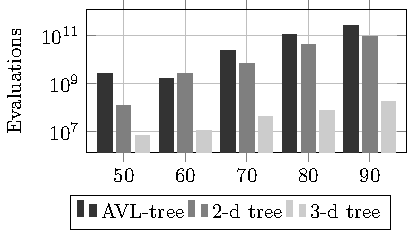
\includegraphics[scale=1.1]{tab/cmp/3dimA}
  \caption{Tipo A}
  \label{fig:sub5}
\end{subfigure}%
\begin{subfigure}{.5\textwidth}
  \centering
  %\begin{tikzpicture}
\begin{axis}[
	x tick label style={ /pgf/number format/1000 sep=},
	width=\cmpW, height=\cmpH,
	ylabel=Evaluations,
	ymode=log,
	grid = both,
	grid style={line width=.0pt, draw=gray!00},
	major grid style={line width=.2pt,draw=gray!50},
	%xlabel=Number of items (n),
	enlargelimits=0.15,
	legend style={at={(\legX,\legY)},
		anchor=north,legend columns=-1},
	ybar=2pt,% configures `bar shift'
	bar width=7pt,
	point meta=y *10^-7, % the displayed number
	cycle list = {black!80,black!50,black!20}
]

\addplot+[fill, text=black]
  coordinates {
    (100,2580591.4)
    (200,367842367.9)
    (300,7975491375.7)
    (400,72030125537.7)
  };

\addplot+[fill, text=black]
  coordinates {
    (100,1571248.6)
    (200,151476739.2)
    (300,2791493175.3)
    (400,45272872459.5)
  };
  
\addplot+[fill, text=black]
  coordinates {
    (100,912878.0)
    (200,29237583.4)
    (300,226471349.8)
    (400,960366212.0)
  };

\legend {AVL-tree,\dtree{2}, \dtree{3}}
\end{axis}
\end{tikzpicture}
  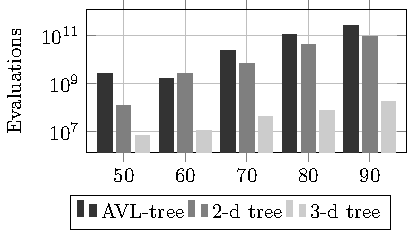
\includegraphics[scale=1.1]{tab/cmp/3dimA}
  \caption{Tipo B}
  \label{fig:sub6}
\end{subfigure}
\begin{subfigure}{.49\textwidth}
  \centering
  %\begin{tikzpicture}
\begin{axis}[
	x tick label style={ /pgf/number format/1000 sep=},
	width=\cmpW, height=\cmpH,
	ylabel=Avaliações,
	ymode=log,
	grid = both,
	grid style={line width=.1pt, draw=gray!00},
	major grid style={line width=.2pt,draw=gray!50},
	%xlabel=Number of items (n),
	enlargelimits=0.15,
	xtick={20, 30, 40},
	xticklabels={20, 30, 40},
	xmin=18,
	xmax=42,
	legend style={at={(\legX,\legY)},
		anchor=north,legend columns=-1},
	ybar=2pt,% configures `bar shift'
	bar width=7pt,
	point meta=y *10^-7, % the displayed number
	cycle list = {black!80,black!50,black!20}
]

\addplot+[fill, text=black]
  coordinates {
    ( 20,221956989)
    ( 30,10861341339)
    ( 40,26505319423)
  };

\addplot+[fill, text=black]
  coordinates {
    ( 20,235426288)
    ( 30,1340276850)
    ( 40,5943925097)
  };
  
\addplot+[fill, text=black]
  coordinates {
    ( 20,1919561)
    ( 30,10225751)
    ( 40,63529280)
  };

\legend {AVL-tree,\dtree{2}, \dtree{3}}
\end{axis}
\end{tikzpicture}

  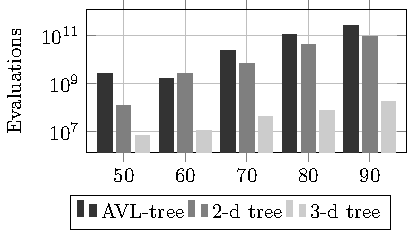
\includegraphics[scale=1.1]{tab/cmp/3dimA}
  \caption{Tipo C}
  \label{fig:sub7}
\end{subfigure}
\begin{subfigure}{.49\textwidth}
  \centering
  %\begin{tikzpicture}
\begin{axis}[
	x tick label style={ /pgf/number format/1000 sep=},
	width=\cmpW, height=\cmpH,
	ylabel=Evaluations,
	ymode=log,
	grid = both,
	grid style={line width=.0pt, draw=gray!00},
	major grid style={line width=.2pt,draw=gray!50},
	%xlabel=Number of items (n),
	enlargelimits=0.15,
	xtick={20, 30},
	xmin=17,
	xmax=33,
	legend style={at={(\legX,\legY)},
		anchor=north,legend columns=-1},
	ybar=2pt,% configures `bar shift'
	bar width=8pt,
	point meta=y *10^-7, % the displayed number
	cycle list = {black!80,black!50,black!20}
]

\addplot+[fill, text=black]
  coordinates {
    (20,481435295.3)
    (30,89269703684.8)
  };

\addplot+[fill, text=black]
  coordinates {
    (20,161607530.0)
    (30,32867842298.12)
  };
  
\addplot+[fill, text=black]
  coordinates {
    (20,2127432.7)
    (30,59136651.9)
  };

\legend {AVL-tree,\dtree{2}, \dtree{3}}
\end{axis}
\end{tikzpicture}
  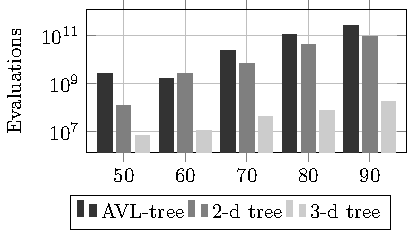
\includegraphics[scale=1.1]{tab/cmp/3dimA}
  \caption{Tipo D}
  \label{fig:sub8}
\end{subfigure}

  \caption{Average number of solution evaluations for 3-objective instances.}
  \label{fig:cmp3dim}
\end{figure}


Table~\ref{tab:cpu3dim} shows results on 3-objective instances for which
were used AVL tree, \dtree{2} and \dtree{3}.
Fig.~\ref{fig:cmp3dim} presents the number of solutions evaluations for 3-objective cases.
Each presented value is the average for 10 instances.

%It can be noted that
The use of multi-dimensional indexing for all 3-objective cases
increased the performance of the algorithm with \dtree{3}
outperforming \dtree{2} on types A, C and D.
The use of \kdtree{} still had lower performance on type B.
